\documentclass[aspectratio=169, 10pt]{beamer}

\usetheme{Madrid}
\usecolortheme{whale}
\usefonttheme{professionalfonts}

\usepackage{amsmath, amssymb, mathtools}
\usepackage{booktabs, tabularx, multirow, makecell}
\usepackage{tikz}
\usetikzlibrary{arrows.meta, shapes.geometric, positioning, fit, backgrounds, decorations.pathreplacing, calc, matrix}
\usepackage{pgfplots}
\pgfplotsset{compat=1.18}
\usepackage{xcolor}
\usepackage{tcolorbox}
\tcbuselibrary{skins, breakable}
\usepackage{graphicx}
\usepackage{adjustbox}
\usepackage{array}
\usepackage{colortbl}
\usepackage{microtype}

\graphicspath{{presentation_assets/}}

\definecolor{deepblue}{HTML}{1A3C6E}
\definecolor{midblue}{HTML}{2E6DB4}
\definecolor{lightblue}{HTML}{D6E8F8}
\definecolor{accentorange}{HTML}{E07B39}
\definecolor{accentgreen}{HTML}{2A7D4F}
\definecolor{accentred}{HTML}{C0392B}
\definecolor{accentpurple}{HTML}{6C3483}
\definecolor{graybg}{HTML}{F4F6F9}
\definecolor{darkgray}{HTML}{3D3D3D}

\setbeamercolor{palette primary}{bg=deepblue, fg=white}
\setbeamercolor{palette secondary}{bg=midblue, fg=white}
\setbeamercolor{palette tertiary}{bg=deepblue!70, fg=white}
\setbeamercolor{titlelike}{bg=deepblue, fg=white}
\setbeamercolor{structure}{fg=deepblue}
\setbeamercolor{block title}{bg=deepblue, fg=white}
\setbeamercolor{block body}{bg=lightblue!50}
\setbeamercolor{block title alerted}{bg=accentred, fg=white}
\setbeamercolor{block body alerted}{bg=accentred!10}
\setbeamercolor{block title example}{bg=accentgreen, fg=white}
\setbeamercolor{block body example}{bg=accentgreen!10}
\setbeamercolor{frametitle}{bg=deepblue, fg=white}
\setbeamercolor{footline}{bg=deepblue!90, fg=white}

\newcommand{\researchbox}[2]{%
  \begin{tcolorbox}[colback=accentorange!10, colframe=accentorange,
    title={\textbf{Research Lens:} #1}, fonttitle=\bfseries\small,
    left=4pt, right=4pt, top=3pt, bottom=3pt, boxrule=1pt]
    \small #2
  \end{tcolorbox}}

\newcommand{\takeawaybox}[2]{%
  \begin{tcolorbox}[colback=accentgreen!10, colframe=accentgreen,
    title={\textbf{Takeaway:} #1}, fonttitle=\bfseries\small,
    left=4pt, right=4pt, top=3pt, bottom=3pt, boxrule=1pt]
    \small #2
  \end{tcolorbox}}

\setbeamertemplate{navigation symbols}{}
\setbeamertemplate{footline}{%
  \leavevmode\hbox{%
    \begin{beamercolorbox}[wd=.33\paperwidth,ht=2.5ex,dp=1.5ex,left,leftskip=4pt]{footline}
      \usebeamerfont{author in head/foot}BTP Research
    \end{beamercolorbox}%
    \begin{beamercolorbox}[wd=.34\paperwidth,ht=2.5ex,dp=1.5ex,center]{footline}
      Graph-Based Discourse Analysis
    \end{beamercolorbox}%
    \begin{beamercolorbox}[wd=.33\paperwidth,ht=2.5ex,dp=1.5ex,right,rightskip=4pt]{footline}
      \insertframenumber/\inserttotalframenumber
    \end{beamercolorbox}%
  }\vskip0pt}

\title[Graph-Based Discourse Analysis]{%
  \textbf{Graph-Based Analysis for Large-Scale Online Discourse}\\[4pt]
  \large From Stance Graph Construction to Graph-Aware and Graph-Context Models}
\subtitle{Problem Setting, Algorithms, Experiments, Benchmarks, and Interpretation}
\author{BTP Research Presentation}
\date{\today}

\begin{document}

\begin{frame}{Title}
  \titlepage
  \vspace{-0.6em}
  \begin{columns}
    \column{0.32\textwidth}
    \begin{tcolorbox}[colback=deepblue!10,colframe=deepblue,boxrule=0.7pt,left=3pt,right=3pt,top=2pt,bottom=2pt]
      \centering\small\textbf{Task}\\\footnotesize Support / Attack / Neutral
    \end{tcolorbox}
    \column{0.32\textwidth}
    \begin{tcolorbox}[colback=accentorange!15,colframe=accentorange,boxrule=0.7pt,left=3pt,right=3pt,top=2pt,bottom=2pt]
      \centering\small\textbf{Dataset}\\\footnotesize SyncIALO
    \end{tcolorbox}
    \column{0.32\textwidth}
    \begin{tcolorbox}[colback=accentgreen!15,colframe=accentgreen,boxrule=0.7pt,left=3pt,right=3pt,top=2pt,bottom=2pt]
      \centering\small\textbf{Best Model}\\\footnotesize Graph-Context
    \end{tcolorbox}
  \end{columns}
\end{frame}

\begin{frame}{Roadmap}
  \tableofcontents
\end{frame}

\section{Problem Setting}

\begin{frame}{Why Large-Scale Online Discourse Needs Graph-Based Analysis}
  \begin{columns}[T]
    \begin{column}{0.56\textwidth}
    Large-scale online discourse is not just a bag of isolated sentences.
    \begin{itemize}
      \item Claims respond to earlier claims.
      \item Multiple speakers form support and attack chains.
      \item Contradictions and circular reasoning emerge across several claims.
      \item Local pairwise predictions do not reveal global argumentative structure.
    \end{itemize}

    In real debate platforms, we therefore need:
    \begin{itemize}
      \item Claim-level relation prediction.
      \item Graph-level structural reasoning.
      \item Interpretable outputs for discourse analysis.
    \end{itemize}

    \researchbox{Core Motivation}{
      The central research challenge is not only to decide whether one claim supports or attacks another, but to build a stance graph reliable enough for downstream graph reasoning.
    }
    \end{column}
    \begin{column}{0.40\textwidth}
      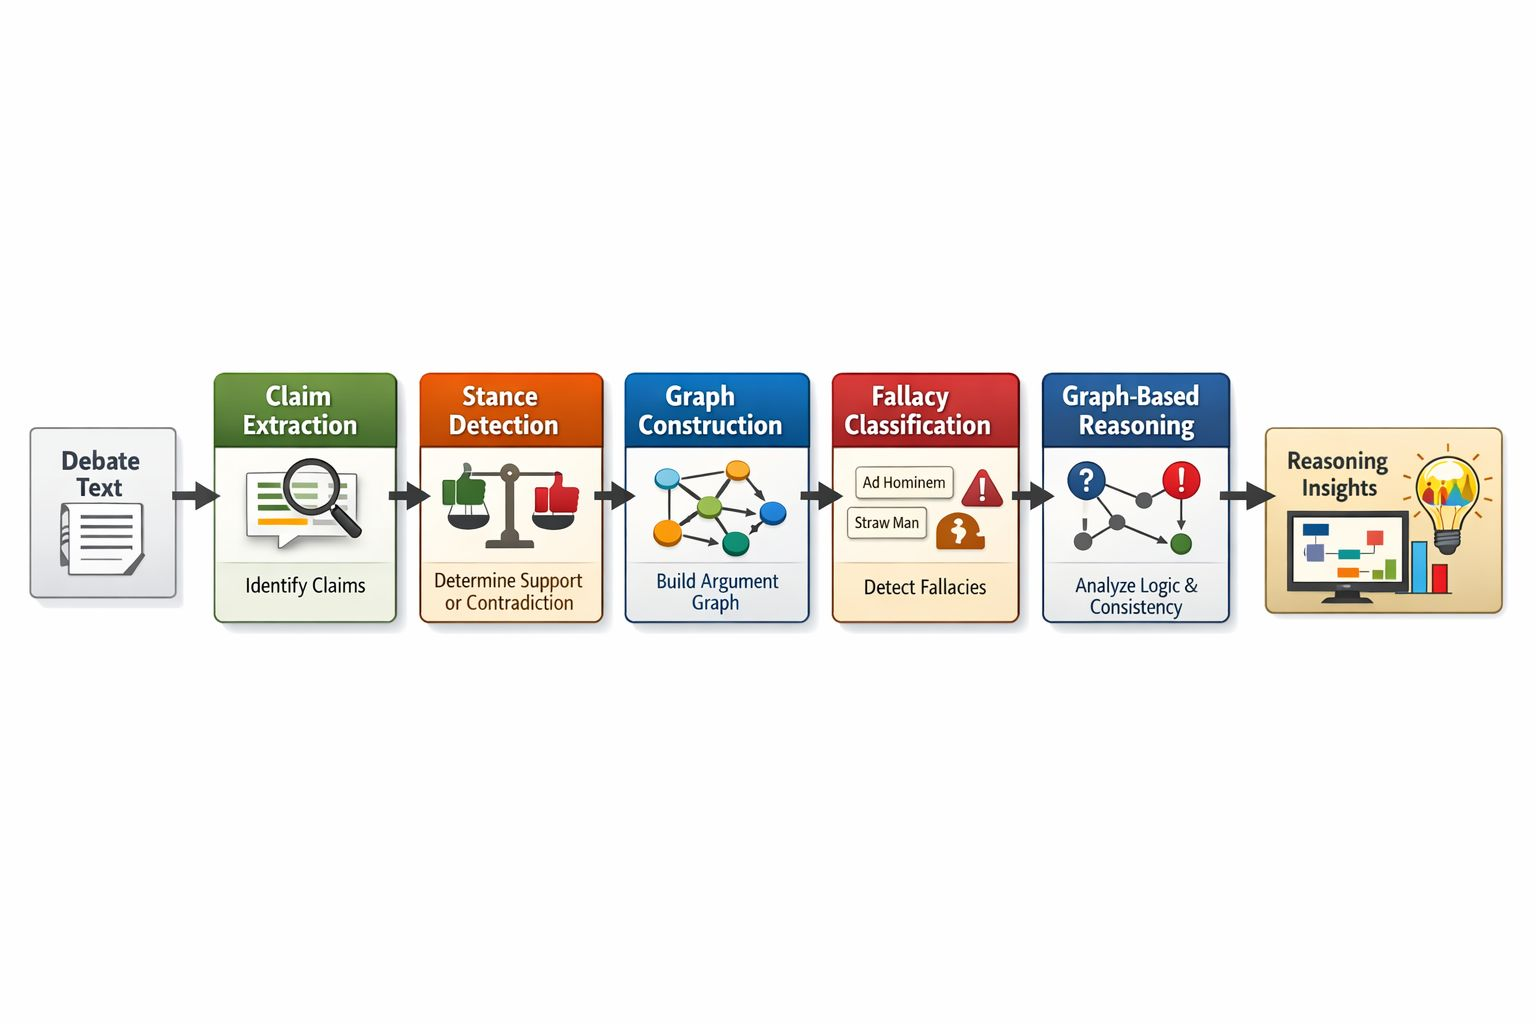
\includegraphics[width=\linewidth]{1.jpg}
    \end{column}
  \end{columns}
\end{frame}

\begin{frame}{Problem Formulation}
Each candidate relation is a directed edge:
\[
e = (u,v,y)
\]
where:
\begin{itemize}
  \item \(u\) is the source claim.
  \item \(v\) is the target claim.
  \item \(y \in \{\texttt{support}, \texttt{attack}, \texttt{neutral}\}\).
\end{itemize}

The modeling convention used throughout the experiments is:
\begin{itemize}
  \item Premise \(=\) target claim text.
  \item Hypothesis \(=\) source claim text.
\end{itemize}

\begin{block}{Research Objective}
Learn accurate edge labels so that the resulting stance graph supports high-quality graph algorithms for discourse analysis.
\end{block}
\end{frame}

\begin{frame}{Why Pairwise Classification Alone Is Not Enough}
Pure pairwise models answer:
\begin{quote}
What do these two claims appear to say to each other?
\end{quote}

But discourse analysis requires harder questions:
\begin{itemize}
  \item Is this claim weakly supported globally?
  \item Does this claim sit inside a contradiction loop?
  \item Is this claim central in a support cluster or an attack hub?
  \item Does this part of the debate fragment into polarized communities?
  \item Which claims act as bridges, bottlenecks, or vulnerable points?
\end{itemize}

\takeawaybox{Why Graphs Matter}{
These are graph questions, not sentence-pair questions. A graph representation is therefore the bridge between local stance detection and global discourse reasoning.
}
\end{frame}

\begin{frame}{End-to-End Research Pipeline}
  \begin{columns}[T]
    \begin{column}{0.53\textwidth}
      \begin{enumerate}
        \item Extract or parse claims.
        \item Predict stance relations between candidate claim pairs.
        \item Construct a directed labeled stance graph.
        \item Run graph algorithms on the predicted graph.
        \item Interpret discourse patterns and structural weaknesses.
      \end{enumerate}

      \vspace{0.5em}
      This presentation focuses on two linked research problems:
      \begin{itemize}
        \item How to construct better stance graphs.
        \item How to reason over them with graph algorithms.
      \end{itemize}
    \end{column}
    \begin{column}{0.43\textwidth}
      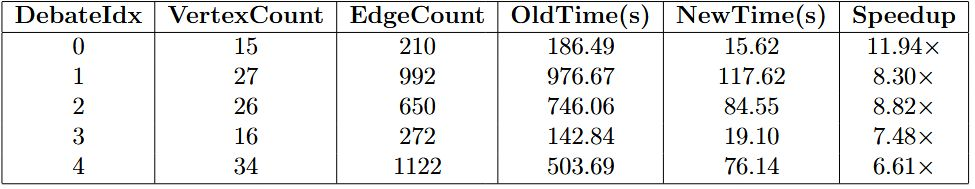
\includegraphics[width=\linewidth]{7.jpg}
    \end{column}
  \end{columns}
\end{frame}

\section{Graph Algorithms}

\begin{frame}{Stance Graph Representation}
Given predicted claim relations, we define the stance graph
\[
G = (V, E_s, E_a, E_n)
\]
where:
\begin{itemize}
  \item \(V\) is the set of claims.
  \item \(E_s\) is the set of support edges.
  \item \(E_a\) is the set of attack edges.
  \item \(E_n\) is the set of neutral candidate relations.
  \item Each non-neutral edge may also carry a confidence weight \(w(u,v)\in[0,1]\).
\end{itemize}

We further use:
\[
G_s = (V,E_s), \qquad G_a = (V,E_a)
\]
for support-only and attack-only analyses.
\end{frame}

\begin{frame}{Graph Algorithm Family: What We Want to Measure}
\begin{itemize}
  \item Contradictions: Where do explicit or structural attacks accumulate?
  \item Circular reasoning: Where do directed cycles emerge?
  \item Support weakness: Which claims receive too little support?
  \item Influence: Which claims dominate support or attack flow?
  \item Vulnerability: Which claims disconnect the reasoning structure if cut?
  \item Community structure: Which claims form coherent clusters or camps?
\end{itemize}

\researchbox{Important Dependency}{
All of these algorithms assume the stance graph is meaningful. If edge labels are noisy, graph reasoning becomes noisy too. That is why the presentation first motivates graph algorithms, and then spends most of its time on improving stance graph construction.
}
\end{frame}

\begin{frame}{Algorithm 1: Contradiction Detection}
Contradiction detection can be defined at the edge level and at the node level.

\textbf{Edge-level contradiction:}
\[
\mathcal{C}_{\text{edge}} = \{(u,v)\in E_a \;:\; w(u,v)\ge \tau\}
\]

\textbf{Node-level contradiction load:}
\[
\mathrm{ContradictLoad}(v) = \sum_{(u,v)\in E_a} w(u,v)
\]

\begin{itemize}
  \item High contradiction load means many claims directly oppose \(v\).
  \item This helps identify contested or vulnerable claims.
  \item In large online discourse, contradiction load reveals where the debate is most polarized.
\end{itemize}
\end{frame}

\begin{frame}{Algorithm 2: Cycle Detection for Circular Reasoning}
Circular reasoning emerges when support relations form a directed cycle:
\[
u_1 \rightarrow u_2 \rightarrow \cdots \rightarrow u_k \rightarrow u_1
\]
with all edges in \(E_s\).

\textbf{Cycle condition:}
\[
\exists \; (u_1,\dots,u_k) \text{ such that } (u_i,u_{i+1})\in E_s,\; (u_k,u_1)\in E_s
\]

\begin{itemize}
  \item If claim \(A\) justifies \(B\), \(B\) justifies \(C\), and \(C\) justifies \(A\), the argument chain becomes self-grounding.
  \item Directed cycle enumeration therefore becomes a structural detector for circular support.
  \item This flaw cannot be found with isolated pair classification alone.
    \end{itemize}
\end{frame}

\begin{frame}{Algorithm 3: Support In-Degree}
The support in-degree of a claim \(v\) is:
\[
d_s^{-}(v) = \sum_{u \in V} \mathbb{I}[(u,v)\in E_s]
\]
or, in weighted form,
\[
\tilde d_s^{-}(v) = \sum_{(u,v)\in E_s} w(u,v)
\]

\begin{itemize}
  \item Low support in-degree indicates a weakly defended claim.
  \item High support in-degree indicates a claim that many other claims reinforce.
  \item This is a simple but useful way to flag weakly supported arguments.
\end{itemize}
\end{frame}

\begin{frame}{Algorithm 4: PageRank on the Support Graph}
Support influence is measured by running PageRank on \(G_s\):
\[
\mathbf{p}_s = \alpha A_s^\top D_s^{-1}\mathbf{p}_s + (1-\alpha)\frac{\mathbf{1}}{|V|}
\]

\begin{itemize}
  \item \(A_s\) is the support adjacency matrix.
  \item \(D_s\) is the support out-degree matrix.
  \item \(\alpha\) is the damping factor.
\end{itemize}

\begin{itemize}
  \item A claim becomes important not only when it has many supporters, but when it is supported by already important claims.
  \item This captures recursive support centrality.
\end{itemize}
\end{frame}

\begin{frame}{Algorithm 5: PageRank on the Attack Graph}
Attack influence is measured analogously on \(G_a\):
\[
\mathbf{p}_a = \alpha A_a^\top D_a^{-1}\mathbf{p}_a + (1-\alpha)\frac{\mathbf{1}}{|V|}
\]

\begin{itemize}
  \item Claims with high attack PageRank act as attack hubs or highly contested targets.
  \item This reveals where opposition concentrates.
  \item Attack centrality is often as informative as support centrality.
\end{itemize}
\end{frame}

\begin{frame}{Algorithm 6: Net Influence}
To summarize whether a claim is overall reinforced or undermined, we define:
\[
\mathrm{NetInf}(v) = \mathbf{p}_s(v) - \lambda \mathbf{p}_a(v)
\]

\begin{itemize}
  \item Positive net influence indicates claims that are support-central and not too attack-central.
  \item Negative net influence indicates claims whose discourse role is dominated by attack pressure.
  \item This creates a single scalar summary of argumentative status.
\end{itemize}
\end{frame}

\begin{frame}{Algorithm 7: Min-Cut Vulnerability}
Given source set \(S\) and target set \(T\), the minimum cut is:
\[
\mathrm{MinCut}(S,T) = \min_{C \subseteq E} \sum_{e\in C} w(e)
\]
such that removing \(C\) disconnects \(S\) from \(T\).

\begin{itemize}
  \item Small cut value means only a few crucial edges keep two argument regions connected.
  \item Such structures are vulnerable bottlenecks.
  \item In debate analysis, this identifies fragile bridges between sub-arguments.
\end{itemize}
\end{frame}

\begin{frame}{Algorithm 8: Clustering and Theme Discovery}
Community structure can be analyzed through support-graph clustering. One common objective is modularity:
\[
Q = \frac{1}{2m}\sum_{i,j}\left(A_{ij} - \frac{k_i k_j}{2m}\right)\delta(c_i,c_j)
\]

After clusters are identified, TF--IDF can summarize cluster themes:
\[
\mathrm{tfidf}(t,c) = \mathrm{tf}(t,c)\cdot \log\!\left(\frac{1+N}{1+\mathrm{df}(t)}\right)
\]

\begin{itemize}
  \item Discover subtopics.
  \item Reveal discourse camps.
  \item Summarize what each cluster is about.
\end{itemize}
\end{frame}

\begin{frame}{How These Algorithms Operate on Stance Graphs}
  \begin{columns}[T]
    \begin{column}{0.53\textwidth}
      The algorithms above are not run on raw text.
      They are run on the predicted stance graph:
      \begin{enumerate}
        \item Claims become nodes.
        \item Support and attack predictions become labeled edges.
        \item Confidence scores become edge weights.
        \item Graph algorithms then read that structure.
      \end{enumerate}

      \begin{block}{Key Dependency}
      Better stance detection produces better stance graphs, which in turn makes the downstream graph algorithms more reliable and more interpretable.
      \end{block}
    \end{column}
    \begin{column}{0.43\textwidth}
      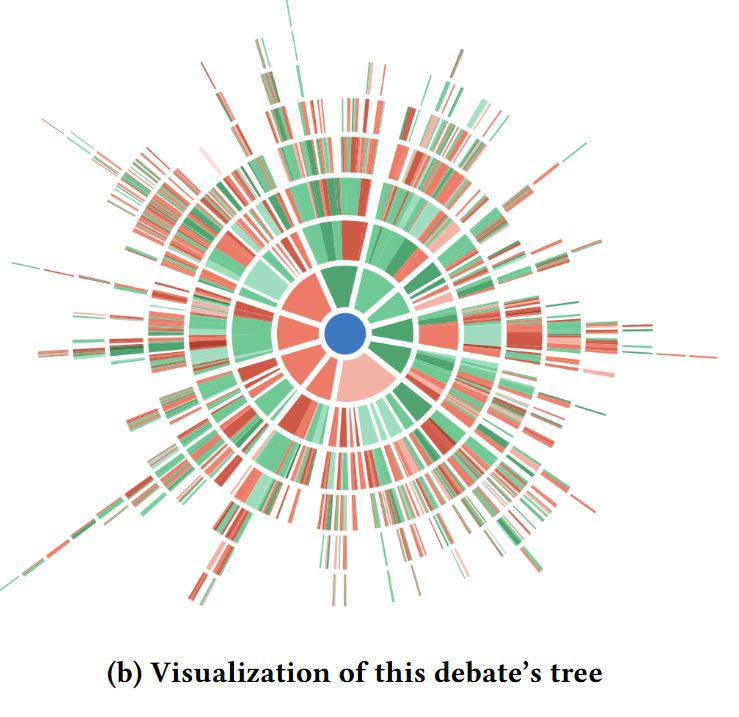
\includegraphics[width=\linewidth]{9.jpg}
    \end{column}
  \end{columns}
\end{frame}

\section{Stance Graph Experiments}

\begin{frame}{Experimental Progression for Building Stance Graphs}
The stance graph construction experiments proceed in four stages:
\begin{enumerate}
  \item Old DeBERTa rule/decision baseline.
  \item Old stance-only baseline.
  \item Meta logistic regression fusion baseline.
  \item Structured models:
  \begin{itemize}
    \item Graph-Aware (graph-statistic-aware).
    \item Graph-Context (graph-ancestor-context-aware).
  \end{itemize}
\end{enumerate}

This sequence isolates where improvement comes from:
\begin{itemize}
  \item Better text modeling.
  \item Better model fusion.
  \item Better structured discourse context.
\end{itemize}
\end{frame}

\begin{frame}{Dataset and Benchmark Protocol}
Saved benchmark configuration:
\begin{itemize}
  \item Dataset: SyncIALO
  \item Corpus: \texttt{synthetic\_corpus-001}
  \item Split: \texttt{eval}
  \item Debates used: \(8\)
  \item Train debates: \(6\)
  \item Test debates: \(2\)
  \item Train examples: \(7224\)
  \item Test examples: \(2664\)
\end{itemize}

Class distribution:
\[
\text{Support}=2472,\qquad \text{Attack}=2472,\qquad \text{Neutral}=4944
\]

Neutral examples are sampled non-edges inside each debate so the final task becomes a three-way edge classification problem.
\end{frame}

\begin{frame}{Experiment 1: DeBERTa Rule/Decision Baseline}
  \begin{columns}[T]
    \begin{column}{0.56\textwidth}
      The first baseline uses a pretrained NLI model directly:
      \[
      \mathbf{x}_{\mathrm{NLI}} =
      [\ell_{\mathrm{contradiction}},\ell_{\mathrm{neutral}},\ell_{\mathrm{entailment}}]
      \]

      A handcrafted decision rule then maps these outputs to:
      \[
      \hat y \in \{\texttt{support},\texttt{attack},\texttt{neutral}\}
      \]

      \textbf{Research role:}
      \begin{itemize}
        \item Establishes whether generic NLI alone can create useful stance graphs.
        \item Tests semantic contradiction and entailment without any debate-specific structure.
      \end{itemize}
    \end{column}
    \begin{column}{0.40\textwidth}
      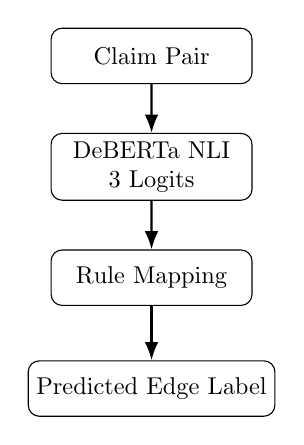
\begin{tikzpicture}[scale=0.88, every node/.style={transform shape}, >=Latex]
        \node[draw, rounded corners, minimum width=2.9cm, minimum height=0.8cm, align=center] (pair) at (0,0) {Claim Pair};
        \node[draw, rounded corners, minimum width=2.9cm, minimum height=0.8cm, align=center] (nli) at (0,-1.6) {DeBERTa NLI\\3 Logits};
        \node[draw, rounded corners, minimum width=2.9cm, minimum height=0.8cm, align=center] (rule) at (0,-3.2) {Rule Mapping};
        \node[draw, rounded corners, minimum width=2.9cm, minimum height=0.8cm, align=center] (out) at (0,-4.8) {Predicted Edge Label};
        \draw[->, thick] (pair) -- (nli);
        \draw[->, thick] (nli) -- (rule);
        \draw[->, thick] (rule) -- (out);
      \end{tikzpicture}
    \end{column}
  \end{columns}
\end{frame}

\begin{frame}{Experiment 1 Results and Interpretation}
\[
\text{Accuracy}=0.5601,\qquad
\text{Macro-F1}=0.3907,\qquad
\text{Weighted-F1}=0.4658
\]

\begin{center}
\begin{tabular}{lccc}
\toprule
Class & Precision & Recall & F1 \\
\midrule
Support & 0.8182 & 0.1081 & 0.1910 \\
Attack & 0.8722 & 0.1742 & 0.2904 \\
Neutral & 0.5338 & 0.9790 & 0.6909 \\
\bottomrule
\end{tabular}
\end{center}

\takeawaybox{Interpretation}{
Generic NLI strongly overpredicts neutral. It recognizes that many pairs are not clearly entailing or contradicting, but it does not yet model debate stance well enough to build a reliable stance graph.
}
\end{frame}

\begin{frame}{Experiment 2: Stance-Only Baseline}
  \begin{columns}[T]
    \begin{column}{0.56\textwidth}
      The second baseline uses a target-dependent stance model directly:
      \[
      \mathbf{x}_{\mathrm{stance}} =
      [\ell_{\mathrm{against}},\ell_{\mathrm{none}},\ell_{\mathrm{favor}}]
      \]

      Prediction is made directly from the stance outputs.

      \textbf{Research role:}
      \begin{itemize}
        \item Tests whether stance supervision alone is better than generic NLI.
        \item Removes NLI but keeps a task-specialized text model.
      \end{itemize}
    \end{column}
    \begin{column}{0.40\textwidth}
      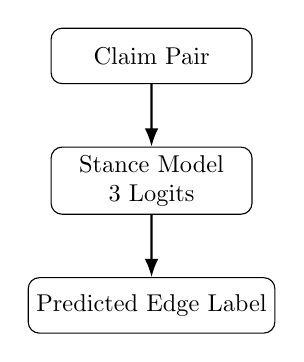
\begin{tikzpicture}[scale=0.88, every node/.style={transform shape}, >=Latex]
        \node[draw, rounded corners, minimum width=2.9cm, minimum height=0.8cm, align=center] (pair) at (0,0) {Claim Pair};
        \node[draw, rounded corners, minimum width=2.9cm, minimum height=0.8cm, align=center] (stance) at (0,-1.8) {Stance Model\\3 Logits};
        \node[draw, rounded corners, minimum width=2.9cm, minimum height=0.8cm, align=center] (out) at (0,-3.6) {Predicted Edge Label};
        \draw[->, thick] (pair) -- (stance);
        \draw[->, thick] (stance) -- (out);
      \end{tikzpicture}
    \end{column}
  \end{columns}
\end{frame}

\begin{frame}{Experiment 2 Results and Interpretation}
\[
\text{Accuracy}=0.3517,\qquad
\text{Macro-F1}=0.3104,\qquad
\text{Weighted-F1}=0.3349
\]

\begin{itemize}
  \item This is the weakest of the core baselines.
  \item The model captures stance sentiment more directly than NLI, but it lacks the richer compatibility structure present in an NLI model.
  \item Used alone, it is not sufficient to support large-scale graph reasoning.
\end{itemize}

\researchbox{Interpretation}{
The result shows that stance cues alone are too brittle. Strong stance graph construction needs both general semantic reasoning and task-specific polarity reasoning.
}
\end{frame}

\begin{frame}{Experiment 3: Meta Logistic Regression Fusion}
  \begin{columns}[T]
    \begin{column}{0.57\textwidth}
      The text-only fusion baseline concatenates the two logit blocks:
      \[
      \mathbf{x}_{\mathrm{base}} =
      [\mathbf{x}_{\mathrm{NLI}};\mathbf{x}_{\mathrm{stance}}]
      \in\mathbb{R}^6
      \]

      A multinomial logistic regression then predicts:
      \[
      P(y=c\mid \mathbf{x}_{\mathrm{base}})
      =
      \frac{\exp(\mathbf{w}_c^\top \mathbf{x}_{\mathrm{base}} + b_c)}
      {\sum_{c'}\exp(\mathbf{w}_{c'}^\top \mathbf{x}_{\mathrm{base}} + b_{c'})}
      \]

      \textbf{Research role:}
      \begin{itemize}
        \item Tests whether a learned fusion of NLI and stance is enough.
        \item Provides the strongest text-only baseline before graph structure is introduced.
      \end{itemize}
    \end{column}
    \begin{column}{0.39\textwidth}
      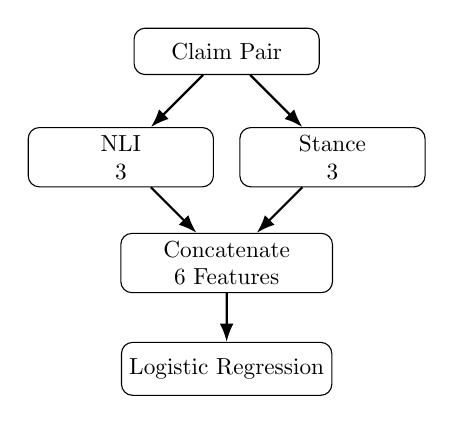
\begin{tikzpicture}[scale=0.84, every node/.style={transform shape}, >=Latex]
        \node[draw, rounded corners, minimum width=2.8cm, minimum height=0.7cm, align=center] (pair) at (0,0) {Claim Pair};
        \node[draw, rounded corners, minimum width=2.8cm, minimum height=0.7cm, align=center] (nli) at (-1.6,-1.6) {NLI\\3};
        \node[draw, rounded corners, minimum width=2.8cm, minimum height=0.7cm, align=center] (stance) at (1.6,-1.6) {Stance\\3};
        \node[draw, rounded corners, minimum width=3.2cm, minimum height=0.8cm, align=center] (fusion) at (0,-3.2) {Concatenate\\6 Features};
        \node[draw, rounded corners, minimum width=3.0cm, minimum height=0.8cm, align=center] (lr) at (0,-4.8) {Logistic Regression};
        \draw[->, thick] (pair) -- (nli);
        \draw[->, thick] (pair) -- (stance);
        \draw[->, thick] (nli) -- (fusion);
        \draw[->, thick] (stance) -- (fusion);
        \draw[->, thick] (fusion) -- (lr);
      \end{tikzpicture}
    \end{column}
  \end{columns}
\end{frame}

\begin{frame}{Experiment 3 Results and Interpretation}
\[
\text{Accuracy}=0.6513,\qquad
\text{Macro-F1}=0.6557,\qquad
\text{Weighted-F1}=0.6477
\]

\begin{itemize}
  \item This is a major jump over the two direct baselines.
  \item It confirms that NLI and stance logits are complementary.
  \item However, the model still only sees isolated pairs.
  \item It has no explicit knowledge of where a claim sits inside the debate.
\end{itemize}

\takeawaybox{Transition}{
The meta logistic model proves that better pairwise fusion helps, but it still does not give us a graph-aware stance graph. That motivates the next stage: structured features derived from the debate itself.
}
\end{frame}

\section{Graph-Aware Model}

\begin{frame}{Why Introduce the Graph-Aware Model}
The Graph-Aware model is the first structured extension beyond text-only fusion.

It asks:
\begin{quote}
Can local semantic graph structure inside a debate improve edge prediction?
\end{quote}

The idea is simple:
\begin{itemize}
  \item Build a debate-local similarity graph.
  \item Derive local graph statistics for each candidate pair.
  \item Fuse these graph features with NLI and stance logits.
\end{itemize}

\researchbox{Core Hypothesis}{
Two claims are easier to classify when the model knows not only what they say to each other, but also whether they occupy the same local semantic region of the debate.
}
\end{frame}

\begin{frame}{Graph-Aware Architecture}
\centering
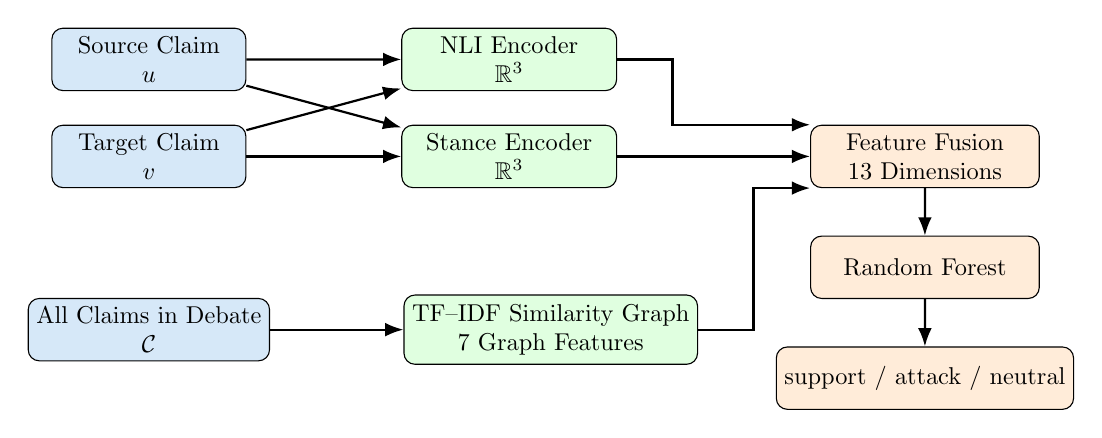
\begin{tikzpicture}[scale=0.88, every node/.style={transform shape}, >=Latex]
  \node[draw, rounded corners, minimum width=2.8cm, minimum height=0.8cm, align=center, fill=lightblue] (src) at (0,2.2) {Source Claim\\\(u\)};
  \node[draw, rounded corners, minimum width=2.8cm, minimum height=0.8cm, align=center, fill=lightblue] (tgt) at (0,0.8) {Target Claim\\\(v\)};
  \node[draw, rounded corners, minimum width=3.2cm, minimum height=0.8cm, align=center, fill=lightblue] (deb) at (0,-1.7) {All Claims in Debate\\\(\mathcal{C}\)};
  \node[draw, rounded corners, minimum width=3.1cm, minimum height=0.9cm, align=center, fill=green!12] (nli) at (5.2,2.2) {NLI Encoder\\\(\mathbb{R}^3\)};
  \node[draw, rounded corners, minimum width=3.1cm, minimum height=0.9cm, align=center, fill=green!12] (stance) at (5.2,0.8) {Stance Encoder\\\(\mathbb{R}^3\)};
  \node[draw, rounded corners, minimum width=3.8cm, minimum height=1.0cm, align=center, fill=green!12] (graph) at (5.8,-1.7) {TF--IDF Similarity Graph\\7 Graph Features};
  \node[draw, rounded corners, minimum width=3.3cm, minimum height=0.9cm, align=center, fill=orange!15] (fusion) at (11.2,0.8) {Feature Fusion\\13 Dimensions};
  \node[draw, rounded corners, minimum width=3.3cm, minimum height=0.9cm, align=center, fill=orange!15] (rf) at (11.2,-0.8) {Random Forest};
  \node[draw, rounded corners, minimum width=3.3cm, minimum height=0.9cm, align=center, fill=orange!15] (pred) at (11.2,-2.4) {support / attack / neutral};
  \draw[->, thick] (src) -- (nli);
  \draw[->, thick] (tgt) -- (nli);
  \draw[->, thick] (src) -- (stance);
  \draw[->, thick] (tgt) -- (stance);
  \draw[->, thick] (deb) -- (graph);
  \draw[->, thick] (nli.east) -- ++(0.8,0) |- (fusion.north west);
  \draw[->, thick] (stance.east) -- (fusion.west);
  \draw[->, thick] (graph.east) -- ++(0.8,0) |- (fusion.south west);
  \draw[->, thick] (fusion) -- (rf);
  \draw[->, thick] (rf) -- (pred);
\end{tikzpicture}
\end{frame}

\begin{frame}[shrink=6]{Graph-Aware Method: Similarity Graph Construction}
For each debate, TF--IDF vectors \(\mathbf{t}_i\) are built for every claim \(c_i\).

The local semantic similarity is:
\[
s(c_i,c_j) = \cos(\mathbf{t}_i,\mathbf{t}_j)
\]

For each claim \(c_i\), the top-\(k\) neighbors above threshold \(\tau\) are retained:
\[
N_k(c_i) = \operatorname{TopK}_{c_j \neq c_i}\left\{s(c_i,c_j): s(c_i,c_j)\ge\tau\right\}
\]

This creates a sparse debate-local semantic graph.

\begin{itemize}
  \item The graph does not encode gold support or attack directly.
  \item It encodes local semantic affinity inside the debate.
  \item The goal is to tell whether two claims live in the same semantic neighborhood.
\end{itemize}
\end{frame}

\begin{frame}[shrink=6]{Graph-Aware Method: The Seven Graph Features}
For candidate edge \((u,v)\), the graph feature vector is:
\[
\mathbf{x}_{\mathrm{graph}}(u,v)=
[f_1,f_2,f_3,f_4,f_5,f_6,f_7]\in\mathbb{R}^7
\]

\[
f_1(u,v)=\cos(\mathbf{t}_u,\mathbf{t}_v)
\]
\[
f_2(u,v)=\frac{|N_k(u)|}{\max(1,k)}, \qquad
f_3(u,v)=\frac{|N_k(v)|}{\max(1,k)}
\]
\[
f_4(u,v)=\mathbb{I}[v\in N_k(u)], \qquad
f_5(u,v)=\mathbb{I}[u\in N_k(v)]
\]
\[
f_6(u,v)=\frac{|N_k(u)\cap N_k(v)|}{|N_k(u)\cup N_k(v)|}
\]
\[
f_7(u,v)=\frac{|T(u)\cap T(v)|}{|T(u)\cup T(v)|}
\]
where \(T(c)\) is the set of tokens in claim \(c\).
\end{frame}

\begin{frame}{Graph-Aware Method: Why These Features Help}
\begin{itemize}
  \item \(\mathbf{f_1}\) Cosine similarity solves the local relevance problem.
  \item \(\mathbf{f_2,f_3}\) Degree features estimate whether the source or target lies in a dense semantic region.
  \item \(\mathbf{f_4,f_5}\) Directed membership captures whether one claim is among the other's strongest neighbors.
  \item \(\mathbf{f_6}\) Neighbor Jaccard overlap checks whether the two claims share the same local neighborhood.
  \item \(\mathbf{f_7}\) Token Jaccard overlap provides a surface lexical overlap signal.
\end{itemize}

\takeawaybox{Important Intuition}{
The Graph-Aware model does not yet reason over argument ancestry. It reasons over local semantic geometry. That is why it is graph-aware, but not yet fully discourse-aware.
}
\end{frame}

\begin{frame}{Graph-Aware Fusion and Decision Rule}
The complete Graph-Aware input is:
\[
\mathbf{x}_{\mathrm{graphfull}} =
[\mathbf{x}_{\mathrm{NLI}};\mathbf{x}_{\mathrm{stance}};\mathbf{x}_{\mathrm{graph}}]
\in\mathbb{R}^{13}
\]

Prediction is made with a Random Forest:
\[
\hat y = \arg\max_{c\in\{\texttt{support},\texttt{attack},\texttt{neutral}\}}
P_{\mathrm{RF}}(c\mid \mathbf{x}_{\mathrm{graphfull}})
\]

\begin{itemize}
  \item NLI captures contradiction and entailment structure.
  \item Stance captures target-dependent polarity.
  \item Graph features capture local semantic placement.
  \item The forest models nonlinear interactions between them.
\end{itemize}
\end{frame}

\begin{frame}{Graph-Aware Results}
\[
\text{Accuracy}=0.8818,\qquad
\text{Macro-F1}=0.8665,\qquad
\text{Weighted-F1}=0.8811
\]

\begin{center}
\begin{tabular}{lccc}
\toprule
Class & Precision & Recall & F1 \\
\midrule
Support & 0.8485 & 0.8243 & 0.8363 \\
Attack & 0.8525 & 0.8243 & 0.8382 \\
Neutral & 0.9111 & 0.9392 & 0.9250 \\
\bottomrule
\end{tabular}
\end{center}

\takeawaybox{Interpretation}{
This is the first model that produces a genuinely strong stance graph. It improves sharply over the text-only fusion baseline by giving the classifier access to local semantic structure.
}
\end{frame}

\begin{frame}{Graph-Aware Confusion Matrix and Error Profile}
\[
\begin{bmatrix}
549 & 56 & 61 \\
56 & 549 & 61 \\
42 & 39 & 1251
\end{bmatrix}
\]

\begin{itemize}
  \item Neutral separation is already strong.
  \item The main residual error is symmetric support-vs-attack confusion.
  \item This means the model is good at deciding whether a pair is relevant, but less certain about exact argumentative polarity.
\end{itemize}
\end{frame}

\begin{frame}{Graph-Aware Feature-Group Ablation}
\begin{center}
\begin{tabular}{lcccc}
\toprule
Subset & Features & Accuracy & Macro-F1 & Weighted-F1 \\
\midrule
\texttt{nli+stance+graph} & 13 & \textbf{0.8799} & \textbf{0.8650} & \textbf{0.8793} \\
\texttt{nli+graph} & 10 & 0.8780 & 0.8620 & 0.8774 \\
\texttt{nli+stance} & 6 & 0.6866 & 0.6710 & 0.6832 \\
\texttt{graph} & 7 & 0.7095 & 0.6363 & 0.7069 \\
\bottomrule
\end{tabular}
\end{center}

\begin{itemize}
  \item Graph features are genuinely strong on their own.
  \item Graph features combine especially well with NLI.
  \item Stance adds value, but the strongest interaction is between NLI and graph locality.
\end{itemize}
\end{frame}

\begin{frame}{Graph-Aware Internal Ablation}
\begin{center}
\begin{tabular}{lcc}
\toprule
Dropped Feature & Macro-F1 & \(\Delta\) Macro-F1 \\
\midrule
\texttt{cosine\_similarity} & 0.8445 & -0.0212 \\
\texttt{normalized\_source\_degree} & 0.8618 & -0.0039 \\
\texttt{source\_in\_target} & 0.8624 & -0.0033 \\
\texttt{target\_in\_source} & 0.8624 & -0.0033 \\
\texttt{neighbor\_jaccard\_overlap} & 0.8645 & -0.0013 \\
\texttt{normalized\_target\_degree} & 0.8653 & -0.0005 \\
\texttt{token\_jaccard\_overlap} & 0.8660 & +0.0002 \\
\bottomrule
\end{tabular}
\end{center}

\takeawaybox{Main Finding}{
Cosine similarity dominates the graph feature family. The Graph-Aware model works, but much of its gain is explained by one very strong semantic-locality signal.
}
\end{frame}

\begin{frame}{Graph-Aware One-Feature-at-a-Time Benchmark}
\begin{center}
\begin{tabular}{lccc}
\toprule
Kept Graph Feature & Accuracy & Macro-F1 & Weighted-F1 \\
\midrule
\texttt{cosine\_similarity} & \textbf{0.8803} & \textbf{0.8645} & \textbf{0.8795} \\
\texttt{token\_jaccard\_overlap} & 0.8202 & 0.8052 & 0.8191 \\
\texttt{target\_in\_source} & 0.8194 & 0.7994 & 0.8155 \\
\texttt{source\_in\_target} & 0.7980 & 0.7784 & 0.7941 \\
\texttt{neighbor\_jaccard\_overlap} & 0.7845 & 0.7657 & 0.7812 \\
\bottomrule
\end{tabular}
\end{center}

\begin{itemize}
  \item One feature, cosine similarity, almost reproduces the whole Graph-Aware model.
  \item This is a powerful clue: the next model should move beyond local closeness and encode richer discourse context.
\end{itemize}
\end{frame}

\section{Graph-Context Model}

\begin{frame}{Why Move from Graph-Aware to Graph-Context}
The Graph-Aware model answers:
\begin{quote}
Are these two claims locally close in the semantic graph?
\end{quote}

The Graph-Context model asks a richer question:
\begin{quote}
How does each claim relate to its own upstream argument history, and how does each claim relate to the other claim's upstream context?
\end{quote}

\begin{itemize}
  \item Local similarity is helpful, but not sufficient.
  \item Debate relations depend on parent-child and ancestor context.
  \item GraphNLI-style reasoning suggests that upstream context matters more than flat neighborhood geometry.
\end{itemize}
\end{frame}

\begin{frame}{Graph-Context Architecture}
\centering
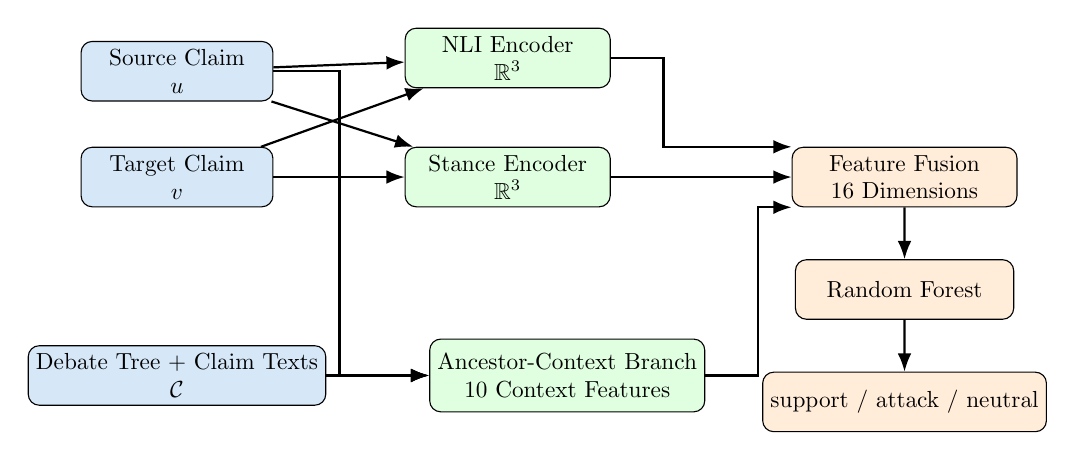
\begin{tikzpicture}[scale=0.84, every node/.style={transform shape}, >=Latex]
  \node[draw, rounded corners, minimum width=2.9cm, minimum height=0.8cm, align=center, fill=lightblue] (src) at (0,2.6) {Source Claim\\\(u\)};
  \node[draw, rounded corners, minimum width=2.9cm, minimum height=0.8cm, align=center, fill=lightblue] (tgt) at (0,1.0) {Target Claim\\\(v\)};
  \node[draw, rounded corners, minimum width=3.5cm, minimum height=0.9cm, align=center, fill=lightblue] (deb) at (0,-2.0) {Debate Tree + Claim Texts\\\(\mathcal{C}\)};
  \node[draw, rounded corners, minimum width=3.1cm, minimum height=0.9cm, align=center, fill=green!12] (nli) at (5.0,2.8) {NLI Encoder\\\(\mathbb{R}^3\)};
  \node[draw, rounded corners, minimum width=3.1cm, minimum height=0.9cm, align=center, fill=green!12] (stance) at (5.0,1.0) {Stance Encoder\\\(\mathbb{R}^3\)};
  \node[draw, rounded corners, minimum width=4.0cm, minimum height=1.1cm, align=center, fill=green!12] (ctx) at (5.9,-2.0) {Ancestor-Context Branch\\10 Context Features};
  \node[draw, rounded corners, minimum width=3.4cm, minimum height=0.9cm, align=center, fill=orange!15] (fusion) at (11.0,1.0) {Feature Fusion\\16 Dimensions};
  \node[draw, rounded corners, minimum width=3.3cm, minimum height=0.9cm, align=center, fill=orange!15] (rf) at (11.0,-0.7) {Random Forest};
  \node[draw, rounded corners, minimum width=3.3cm, minimum height=0.9cm, align=center, fill=orange!15] (pred) at (11.0,-2.4) {support / attack / neutral};
  \draw[->, thick] (src) -- (nli);
  \draw[->, thick] (tgt) -- (nli);
  \draw[->, thick] (src) -- (stance);
  \draw[->, thick] (tgt) -- (stance);
  \draw[->, thick] (deb) -- (ctx);
  \draw[->, thick] (src.east) -- ++(1.0,0) |- (ctx.west);
  \draw[->, thick] (tgt.east) -- ++(1.0,0) |- (ctx.west);
  \draw[->, thick] (nli.east) -- ++(0.8,0) |- (fusion.north west);
  \draw[->, thick] (stance.east) -- (fusion.west);
  \draw[->, thick] (ctx.east) -- ++(0.8,0) |- (fusion.south west);
  \draw[->, thick] (fusion) -- (rf);
  \draw[->, thick] (rf) -- (pred);
\end{tikzpicture}
\end{frame}

\begin{frame}[shrink=4]{Graph-Context Method: Ancestor Construction and TF--IDF}
Each debate induces a tree through the gold reply structure.

For a claim \(c\):
\begin{itemize}
  \item \(a(c)\) is its parent.
  \item \(A(c)=[a_1(c),a_2(c),\dots,a_m(c)]\) is its ancestor sequence.
  \item \(d(c)\) is its depth.
\end{itemize}

Debate-local TF--IDF vectors \(\mathbf{t}_i\) are built as:
\[
\mathrm{tfidf}(t,c_i,\mathcal{C}) = \mathrm{tf}(t,c_i)\cdot
\log\left(\frac{1+|\mathcal{C}|}{1+|\{c\in\mathcal{C}: t\in c\}|}\right)+1
\]

\begin{itemize}
  \item TF--IDF is fit per debate, not globally.
  \item The goal is to measure salience inside the local discourse context.
\end{itemize}
\end{frame}

\begin{frame}[shrink=5]{Graph-Context Method: Weighted Ancestor Context}
For ancestor sequence
\[
A(c)=[a_1(c),a_2(c),\dots,a_m(c)]
\]
we assign exponentially decaying weights:
\[
w_r = \frac{1}{2^{r-1}}, \qquad r=1,\dots,m
\]

The weighted ancestor-context embedding is:
\[
\mathbf{z}(c)=
\frac{\sum_{r=1}^{m} w_r \mathbf{t}_{a_r(c)}}{\sum_{r=1}^{m} w_r}
\]

\begin{itemize}
  \item The parent matters most.
  \item The grandparent matters less.
  \item Farther ancestors still contribute, but with reduced weight.
\end{itemize}

\takeawaybox{Core Idea}{
The Graph-Context model does not just ask whether two claims are close. It asks whether each claim is coherent with the argument history that led to it.
}
\end{frame}

\begin{frame}[shrink=8]{Graph-Context Method: The Ten Context Features}
The context feature vector is:
\[
\mathbf{x}_{\mathrm{context}}(u,v)=[g_1,\dots,g_{10}]\in\mathbb{R}^{10}
\]

\[
g_1=\frac{d(u)}{\max(1,d_{\max})},\quad
g_2=\frac{d(v)}{\max(1,d_{\max})},\quad
g_3=|g_1-g_2|
\]
\[
g_4=\frac{|A(u)|}{\max(1,d_{\max})},\qquad
g_5=\frac{|A(v)|}{\max(1,d_{\max})}
\]
\[
g_6=\cos(\mathbf{t}_u,\mathbf{z}(u)),\qquad
g_7=\cos(\mathbf{t}_v,\mathbf{z}(v))
\]
\[
g_8=\cos(\mathbf{t}_u,\mathbf{z}(v)),\qquad
g_9=\cos(\mathbf{t}_v,\mathbf{z}(u))
\]
\[
g_{10}=\cos(\mathbf{z}(u),\mathbf{z}(v))
\]
\end{frame}

\begin{frame}{Graph-Context Method: Why These Features Matter}
\begin{itemize}
  \item \(g_1,g_2,g_3\) capture where claims lie in the argument tree.
  \item \(g_4,g_5\) capture how much upstream context is available.
  \item \(g_6,g_7\) test whether a claim agrees with its own ancestor history.
  \item \(g_8,g_9\) test cross-context coherence.
  \item \(g_{10}\) compares the two ancestor contexts directly.
\end{itemize}

\researchbox{Why This Is Stronger}{
These features are no longer just geometric. They explicitly encode discourse ancestry, contextual coherence, and cross-context interaction.
}
\end{frame}

\begin{frame}{Graph-Context Fusion and Decision Rule}
The full Graph-Context representation is:
\[
\mathbf{x}_{\mathrm{full}}=
[\mathbf{x}_{\mathrm{NLI}};\mathbf{x}_{\mathrm{stance}};\mathbf{x}_{\mathrm{context}}]
\in\mathbb{R}^{16}
\]

Prediction is again made with a Random Forest:
\[
\hat y = \arg\max_{c}
P_{\mathrm{RF}}(c\mid \mathbf{x}_{\mathrm{full}})
\]

\begin{itemize}
  \item NLI and stance still provide pairwise semantics.
  \item The context branch provides discourse-tree structure.
  \item The forest learns nonlinear interactions between pairwise semantics and upstream context.
\end{itemize}
\end{frame}

\begin{frame}{Graph-Context Results}
\[
\text{Accuracy}=0.9433,\qquad
\text{Macro-F1}=0.9244,\qquad
\text{Weighted-F1}=0.9433
\]

\begin{center}
\begin{tabular}{lccc}
\toprule
Class & Precision & Recall & F1 \\
\midrule
Support & 0.8884 & 0.8844 & 0.8864 \\
Attack & 0.8849 & 0.8889 & 0.8869 \\
Neutral & 1.0000 & 1.0000 & 1.0000 \\
\bottomrule
\end{tabular}
\end{center}

\takeawaybox{Interpretation}{
The Graph-Context model is not just better overall. It produces cleaner support and attack balance and perfect neutral separation on the saved benchmark split.
}
\end{frame}

\begin{frame}{Graph-Context Confusion Matrix and Error Profile}
\[
\begin{bmatrix}
589 & 77 & 0 \\
74 & 592 & 0 \\
0 & 0 & 1332
\end{bmatrix}
\]

\begin{itemize}
  \item Neutral is perfectly separated.
  \item The only remaining errors are support-vs-attack confusions.
  \item This is exactly what we would expect once the model learns discourse relevance and still fine-tunes polarity.
\end{itemize}
\end{frame}

\begin{frame}{Graph-Context Feature-Group Ablation}
\begin{center}
\begin{tabular}{lcccc}
\toprule
Subset & Features & Accuracy & Macro-F1 & Weighted-F1 \\
\midrule
\texttt{nli+stance+context} & 16 & \textbf{0.9441} & \textbf{0.9254} & \textbf{0.9441} \\
\texttt{nli+context} & 13 & 0.9414 & 0.9219 & 0.9414 \\
\texttt{context} & 10 & 0.7815 & 0.7087 & 0.7584 \\
\texttt{nli+stance} & 6 & 0.6866 & 0.6710 & 0.6832 \\
\bottomrule
\end{tabular}
\end{center}

\begin{itemize}
  \item The context family is intrinsically strong.
  \item Context pairs especially well with NLI.
  \item The full model is not just a bigger feature budget. It is a more informative feature family.
\end{itemize}
\end{frame}

\begin{frame}{Graph-Context Internal Ablation}
\begin{center}
\begin{tabular}{lcc}
\toprule
Dropped Context Feature & Macro-F1 & \(\Delta\) Macro-F1 \\
\midrule
\texttt{target\_to\_source\_ancestor\_context} & 0.9215 & -0.0040 \\
\texttt{normalized\_target\_ancestor\_count} & 0.9229 & -0.0025 \\
\texttt{normalized\_source\_depth} & 0.9239 & -0.0015 \\
\texttt{source\_to\_target\_ancestor\_context} & 0.9284 & +0.0030 \\
\bottomrule
\end{tabular}
\end{center}

\begin{itemize}
  \item The strongest context feature is cross-context similarity from target to source context.
  \item The predictive value is more distributed than in Graph-Aware.
  \item This means the Graph-Context model is less fragile and less dominated by one scalar feature.
\end{itemize}
\end{frame}

\begin{frame}{Graph-Context One-Feature-at-a-Time Benchmark}
\begin{center}
\begin{tabular}{lcc}
\toprule
Kept Context Feature & Macro-F1 & Accuracy \\
\midrule
\texttt{target\_to\_source\_ancestor\_context} & \textbf{0.9299} & \textbf{0.9474} \\
\texttt{ancestor\_context\_to\_ancestor\_context} & 0.9204 & 0.9373 \\
\texttt{normalized\_depth\_gap} & 0.7741 & 0.7815 \\
\bottomrule
\end{tabular}
\end{center}

\takeawaybox{Main Finding}{
One carefully chosen ancestor-context feature already outperforms the full Graph-Aware model. That is the clearest evidence that upstream discourse context is more informative than flat graph statistics alone.
}
\end{frame}

\section{Comparison}

\begin{frame}{Overall Benchmark Comparison}
\begin{center}
\begin{tabular}{lccc}
\toprule
Model & Accuracy & Macro-F1 & Weighted-F1 \\
\midrule
DeBERTa Baseline & 0.5601 & 0.3907 & 0.4658 \\
Stance Baseline & 0.3517 & 0.3104 & 0.3349 \\
Meta Logistic & 0.6513 & 0.6557 & 0.6477 \\
Graph-Aware & 0.8818 & 0.8665 & 0.8811 \\
\textbf{Graph-Context} & \textbf{0.9433} & \textbf{0.9244} & \textbf{0.9433} \\
\bottomrule
\end{tabular}
\end{center}

\[
\Delta \text{Macro-F1}_{\text{Graph-Context vs Graph-Aware}}
= 0.9244 - 0.8665 \approx 0.0579
\]
\end{frame}

\begin{frame}{Metric Comparison Bar Chart}
\centering
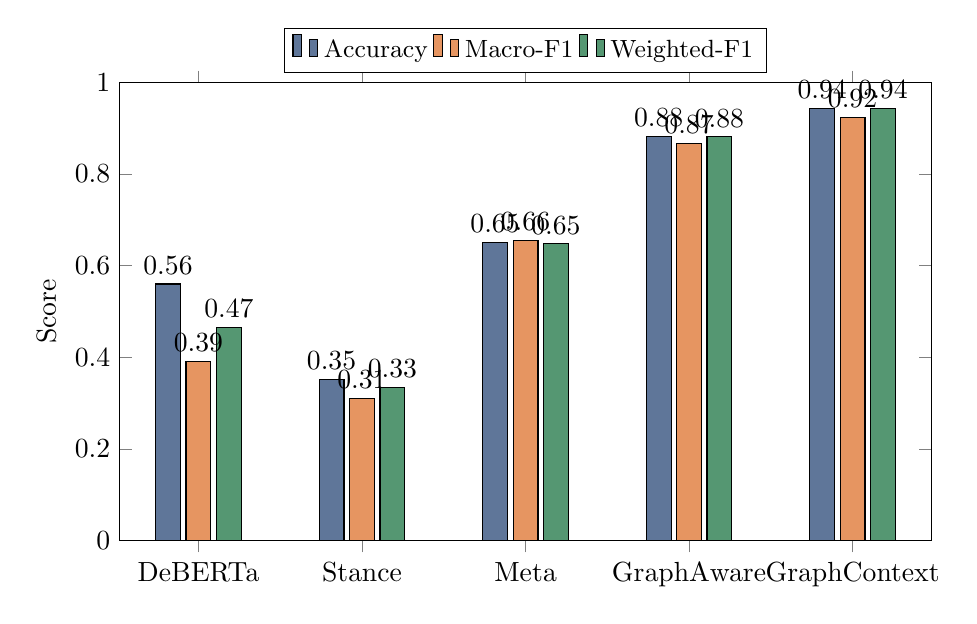
\begin{tikzpicture}
\begin{axis}[
  ybar,
  bar width=9pt,
  width=0.98\textwidth,
  height=7.4cm,
  ymin=0,
  ymax=1.0,
  ylabel={Score},
  symbolic x coords={DeBERTa,Stance,Meta,GraphAware,GraphContext},
  xtick=data,
  legend style={at={(0.5,1.02)},anchor=south,legend columns=3,font=\small},
  nodes near coords,
  nodes near coords align={vertical},
  enlarge x limits=0.12
]
\addplot[fill=deepblue!70] coordinates {
  (DeBERTa,0.5601) (Stance,0.3517) (Meta,0.6513) (GraphAware,0.8818) (GraphContext,0.9433)
};
\addplot[fill=accentorange!80] coordinates {
  (DeBERTa,0.3907) (Stance,0.3104) (Meta,0.6557) (GraphAware,0.8665) (GraphContext,0.9244)
};
\addplot[fill=accentgreen!80] coordinates {
  (DeBERTa,0.4658) (Stance,0.3349) (Meta,0.6477) (GraphAware,0.8811) (GraphContext,0.9433)
};
\legend{Accuracy, Macro-F1, Weighted-F1}
\end{axis}
\end{tikzpicture}
\end{frame}

\begin{frame}{Direct Structured Comparison: Graph-Aware vs Graph-Context}
\begin{center}
\begin{tabular}{lccc}
\toprule
Structured Family & Structured Only & NLI + Structured & NLI + Stance + Structured \\
\midrule
Graph-Aware & 0.6363 & 0.8620 & 0.8650 \\
\textbf{Graph-Context} & \textbf{0.7087} & \textbf{0.9219} & \textbf{0.9254} \\
\bottomrule
\end{tabular}
\end{center}

\begin{itemize}
  \item Graph-Context is stronger as a standalone structured family.
  \item Graph-Context is stronger as a complement to NLI.
  \item Graph-Context remains stronger in the full fused model.
\end{itemize}
\end{frame}

\begin{frame}{Direct Ablation Comparison}
\begin{center}
\begin{tabular}{lcc}
\toprule
Model Family & Most Damaging Dropped Feature & \(\Delta\) Macro-F1 \\
\midrule
Graph-Aware & \texttt{cosine\_similarity} & -0.0212 \\
\textbf{Graph-Context} & \texttt{target\_to\_source\_ancestor\_context} & \textbf{-0.0040} \\
\bottomrule
\end{tabular}
\end{center}

\begin{itemize}
  \item Graph-Aware is highly effective, but dominated by one feature.
  \item Graph-Context spreads useful signal across several features.
  \item The newer model is therefore both stronger and more robust.
\end{itemize}
\end{frame}

\begin{frame}{What Each Structured Model Really Learns}
Graph-Aware mainly answers:
\begin{quote}
Are these two claims locally close in the semantic graph?
\end{quote}

Graph-Context answers:
\begin{quote}
How does each claim relate to its own upstream argument history, and how do the two argument histories interact?
\end{quote}

\takeawaybox{Final Comparison}{
The improvement from Graph-Aware to Graph-Context is not just more features. It is a shift from local semantic geometry to explicit discourse-context modeling.
}
\end{frame}

\section{Conclusion}

\begin{frame}{Conclusion}
\begin{itemize}
  \item Large-scale online discourse requires graph-based analysis because many reasoning patterns are global, not local.
  \item Graph algorithms such as contradiction detection, cycle detection, PageRank, min-cut, and clustering provide a powerful discourse-analysis toolkit.
  \item These algorithms only become useful if the stance graph is reliable.
  \item DeBERTa, stance-only, and meta logistic baselines progressively improve pairwise edge prediction.
  \item The Graph-Aware model is the first strong structured model and shows that debate-local graph statistics help substantially.
  \item The Graph-Context model is stronger still because it encodes upstream discourse ancestry and cross-context coherence.
\end{itemize}
\end{frame}

\begin{frame}{Future Work}
\begin{itemize}
  \item Evaluate on more debates and multiple random seeds.
  \item Extend the Graph-Context model to a true neural graph architecture.
  \item Replace TF--IDF ancestor embeddings with transformer-based contextual embeddings.
  \item Study transfer to CreateDebate and other online discourse corpora.
  \item Build hybrid models that combine graph statistics and ancestor context in a more structured way.
  \item Use improved stance graphs to strengthen downstream contradiction and fallacy detection.
\end{itemize}

\begin{block}{Closing Statement}
The main contribution of this research is the demonstration that better discourse graphs come from better stance modeling, and better stance modeling comes from treating claims as parts of a structured argument graph rather than isolated text pairs.
\end{block}
\end{frame}

\begin{frame}{Thank You}
\centering
\Huge Thank You

\vspace{1em}
\Large Questions and Discussion
\end{frame}

\end{document}
